\chapter{Konzept} \label{chap:Konzept}
In diesem Kapitel soll das Konzept dieser Ausarbeitung vorgestellt werden. Dieses besteht aus vier Teilen. Zuerst soll das Vorgehen erklärt werden, gefolgt von der Darstellung des Environments und der Agenten. Danach soll im weiteren auf die Datenerhebung eingegangen werden.\\
Ziel dieses Abschnittes ist es das Vorgehen und alle weiteren dazu benötigten Elemente unabhängig von der Implementierung darzustellen, sodass die Ergebnisse mit jeder Implementierung reproduzierbar sind.

\section{Vorgehen} \label{sec:Konzept_Vorgehen}
Das Vorgehen lässt sich am besten mit Hilfe eines Flussdiagramms darstellen, in welchem die einzelnen Schritte des Vergleichs visuell dargestellt sind.\\
Zu Beginn sei erwähnt, dass davon ausgegangen wird, dass alle für den Verglich benötigten Komponenten, wie z.B. Environment, Agenten und statistische Analysekomponenten entsprechende der Anforderungen \ref{chap:Anforderungen} implementiert sind.\\
Als erstes werden die Agenten erstellt \ref{fig:Vorgehen}. Für diese Initialisierung werden die Hyperparameter aus \ref{sec:Konzept_Agenten} verwendet.
Mit diesem Baseline Agenten Bestand werden nun die weiteren Vergleich durchgeführt.\\
Für jedes Evaluationskriterien werden aus dem gegebenen Agenten-Bestand die zwei optimalen Baseline Agenten ausgewählt. Die Algorithmus-Art besitzt dabei der Auswahl der Agenten keinen Einfluss. Genauere Details zur Durchführung der Baseline Vergleiche finden sich in \ref{sec:Konzept_Datenerhebung}.\\
Basierend auf den beiden Sieger Agenten (Agent-01 und Agent-02) \ref{fig:Vorgehen}, werden nun die Optimierungen auf das Env. und die Agenten angewendet. Mit diesen optimierten Agenten (Agent-01 Optimierung A bis Agent-02 Optimierung C) werden nun die Vergleiche bezüglich jedes einzelnen Evaluationskriteriums \ref{tab:Kriterien} wiederholt.\\
Im letzten Schritt soll in der gesamt Evaluation der optimale Agent für jedes Evaluationskriterium ermittelt werden. Dabei können dies auch Baseline Agenten sein.
\begin{figure}[H]
	\centering
	\def\svgscale{0.095}
	\chapter{Vorgehen} \label{chap:Vorgehen}
In diesem Kapitel soll das weitere Vorgehen thematisiert werden. Dazu erfolgt eine genaue Erklärung der weiteren Schritte.

\section{Bestimmung der Netzstruktur}

	\caption[Flussdiagramm des Vorgehens]{Darstellung des Vorgehens.}
	\label{fig:Vorgehen}
\end{figure}

\section{Environment} \label{sec:Konzept_Environment}
Das Env besteht im wesentlichen aus einer Hauptkomponenten (Wrapper), welche benötigt wird, um die in \ref{sec:Anforderungen_Schnittstelle} aufgestellten Anforderung zu erfüllen. Diese Hauptkomponente beinhaltet die Spiellogik-Komponente, welche aus fünf weiteren Unterkomponenten besteht.
Zu diesen gehören die Game-, Player-, Reward-, Observation- und GUI-Komponenten.

\subsection{Wrapper} \label{sec:Konzept_Wrapper}
Der Wrapper oder auch die Verbindungskomponente verbindet alle bereits erwähnten Komponenten miteinander. Zu diesem Zweck muss er einige Funktionalitäten implementieren. Diese beziehen sich auf die im Wrapper vorhandenen Komponenten.
\begin{figure}[H]
	\centering
	\def\svgscale{0.15}
	\input{Abbildungen/Wrapper.pdf_tex}
	\caption[Wrapper]{Darstellung des Wrappers.}
	\label{fig:Wrapper}
\end{figure}
Die step Funktionalität \ref{fig:Wrapper} ist die Hauptmethode im Wrapper. Sie bekommt eine Aktion übergeben, welche zuvor vom Agent bestimmt wurde. Diese wird mit Hilfe der Spiellogik umgesetzt. Entsprechend der Anforderung \ref{sec:Anforderungen_Schnittstelle} gibt diese Methode nur einen Reward und eine Obs zurück.\\
Reset setzt den bereits vorhandenen Spielfortschritt zurück, wobei auf die Spiellogikkomponente zugegriffen wird. Die Anforderung \ref{sec:Anforderung_Reset} ist damit erfüllt.\\
Die Render Methode ist für die Visualisierung verantwortlich und ruft Methoden in der GUI-Unterkomponente auf, welche ein genaues Bild von der Spiellogik-Komponente erhält. Die Anforderung \ref{sec:visualisierung_Env} ist damit erfüllt.\\
Die has\_won und has\_ended Methodiken geben Statusinformationen über den Momentanen Spielstand zurück, welche für den Spiel- bzw. Trainingsablauf benötigt werden.

\subsection{Spiellogik} \label{sec:Konzept_Spiellogik}
Die Spiellogik besteht aus den fünf Unterkomponenten, welche in \ref{sec:Konzept_Environment} bereits benannt wurden.\\
Die Game-Komponente ist die wichtigste Komponente von allen, da sie die eigentliche Aktionsdurchführung implementiert. Sie beinhaltet jeweils Instanzen der Reward-, Observation-, GUI- und Player-Komponenten. Letztere ist eine Datenhaltungskomponente, welche die Daten der Snake, wie z.B. Position oder Ausrichtung (Direction) beinhaltet.\\
\\Die Reward-Komponente bestimmt den auszugebenden Reward nach jeder Aktionsabfertigung. Dieser berechnet sich wie in \ref{sec:Konzept_Reward} angegeben. Zuzüglich wird im Rahmen eine der Optimierungen, siehe \ref{sec:Konzept_Vorgehen}, eine weitere Reward Funktion implementiert. Diese berechnet sich wie in \ref{sec:Konzept_Optimierung02} angegeben.\\
\\In der Game-Komponente werden wichtige Spielbezogene Daten verwaltet. Zu diesen gehören das Spielfeld (ground), sowie die Form des Spielfeldes (shape) und die Position des Apfels auf dem Spielfeld. Sie beinhaltet viele Methoden, wie z.B. die action, observe, evaluate, reset, view, make\_apple.
\\In der Player-Komponente, welche zur Datenverwaltung dient, werden Spielerbezogene Daten verwaltet. Zu diesen zählen die Position des Kopfes der Snake, sowie ihrer Schwanzglieder, ihre Ausrichtung (Direction), ihre gelaufenen Schritte seit dem letzten Fressen eines Apfels (inter\_apple\_steps), ihr Lebensstatus (done), daher ob sie tot oder lebendig ist und weitere Farbkonstanten für die GUI.\\
\\Die Observation-Komponente beinhaltet viele einzelne Funktionen zur schrittweisen Erstellung der Observation, wie sie in \ref{sec:Konzept_Observation} erklärt wird.
\\Zur Erzeugung der grafischen Oberfläche implementiert die GUI-Komponente die Funktionalität ein Fenster zu öffnen, welches das Spielgeschehen, daher das Spielfeld (ground) anzeigt und stetig an den neusten Stand anpasst.
\begin{figure}[H]
	\centering
	\def\svgscale{0.17}
	\input{Abbildungen/Spiellogik.pdf_tex}
	\caption[Spiellogik]{Darstellung der Spiellogik mit ihren Unterkomponenten.}
	\label{fig:Spiellogik}
\end{figure}

\subsubsection{Spielablauf} \label{sec:Konzept_Spielablauf}
Die eigentliche Aktionsabarbeitung wird durch das Aufrufen der step Funktionalität im Wrapper \ref{sec:Konzept_Wrapper} bewirkt. Diese ruft die evaluate und observe Methoden auf, welche in der Game-Komponente implementiert sind \ref{fig:Spiellogik}.
Um jedoch zuerst die Abarbeitung einer Aktion durchzuführen, muss die action Methode als aller erste aufgerufen werden, welche die von Agenten bestimmte Aktion (action) übergeben bekommt. 
\begin{figure}[H]
	\centering
	\def\svgscale{0.105}
	\input{Abbildungen/Spielablauf.pdf_tex}
	\caption[Spielablauf]{Darstellung eines Schrittes in der Spielepisode.}
	\label{fig:Spielablauf}
\end{figure}
Zu Beginn wird überprüft, ob die Snake seit dem letzten Fressen mehr Schritte als die eigentliche Spielfeldgröße gegangen ist. Die Spielfeldgröße berechnet sich dabei wie folgt (8, 8) = 64, daher ist die Spielfeldgröße 64. Sollte die Snake mehr Schritte gelaufen sein als diese Größe, so wird das Spiel terminiert, da die Snake eventuell in einer Schleife steckt und daher diese nie wieder verlassen würde.\\
Andernfalls wird die Aktion verarbeitet, in dem sie die direction verändert der Snake manipuliert. Das Spiel Snake besitzt in diesem Konzept drei Actions turn left, turn right oder do nothing.
\begin{longtable}[h]{|p{4cm}|p{\linewidth - 5cm}|}
	\caption{Kodierung der Actions}
	\label{tab:Aktionscodierung} 
	\endfirsthead
	\endhead
	\hline
	Action & Erklärung \\
	\hline
	turn left & Die Snake ändert ihre Richtung um 90° nach links. Z.B. Von N $\longrightarrow$ W \\
	\hline
	turn right & Snake ändert ihre Richtung um 90° nach rechts. Z.B. Von N $\longrightarrow$ O \\
	\hline
	do nothing & Die Richtung der Snake wird nicht verändert. \\
	\hline
\end{longtable}
Entsprechend der Beispiele in \ref{tab:Aktionscodierung} wird klar, dass die Direktion entweder nur Norden, Osten, Süden oder Westen sein kann.
Als nächstes wird ein Schritt der Snake mit der aktualisierten Aktion hypothetisch durchgeführt. Dabei lässt sich feststellen, ob die Ausführung des Schrittes zum Tod der Snake führt. Sollte dies der Fall sein, so wird der Spielablauf terminiert. Dabei führt das laufen in sich selbst und das Verlassen des Spielfeldes zum Tod \ref{sec:Snake}. \\ 
Anderenfalls wird der Schritt durchgeführt. Dabei wird zwischen zwei Fällen unterschieden. Sollte die Snake einen Apfel gefressen haben, also der Kopf der Snake und der Apfel die selbe Position einnehmen, so wächst die Snake um ein Schwanzglied. Der alte Apfel wird entfernt und ein neuer erscheint zufallsbasiert irgendwo auf einem freien Platz des Spielfelds.\\
Sollte die Snake hingegen keinen Apfel gefressen haben, so geht sie einfach den Schritt, es bewegen sich daher Alle Schwanzglieder auf die Vorgängerposition, mit Ausnahme des Kopfes, welcher die, durch die direktion definierte, neue Position einnimmt.\\
Nach der Ausführung einer dieser beiden Fälle, wird die GUI aktualisiert mit der update\_gui Methode. Nach diesem Schritt ist die Abarbeitung der action Methode abgeschlossen. Damit jedoch die der Agent den Nachfolgezustand und Reward erhält wird die evaluate Methode in der Reward-Komponente und die observe Methode in der Observation-Komponente aufgerufen.\\
Zum Schluss werden Obs und Reward zurückgegeben.

\subsubsection{Reward} \label{sec:Konzept_Reward}
Die evaluate Methode befindet sich in der Game-Komponente und ruft ihrerseits die standard\_reward Method in der Reward-Komponente auf. Sie bestimmt, basierend auf dem letzten Zug, den Reward, was nach folgenden Vorbild geschieht.
Der Reward ist abhängig von drei Faktoren. Dem Fressen eines Apfels, dem Sieg und dem Verlust. Sollte keiner dieser genannten Faktoren eintreten, wird ein Reward von -0.01 zurückgegeben. Dies hält den Agenten dazu an den kürzesten Pfad zum Apfel zu finden, da jeder Schritt geringfügig bestraft wird.\\
War es der Snake möglich einen Apfel zu fressen so wird ein Reward von +1.0 zurückgegeben, da ein Sub-Goal erfüllt worden ist.
Sollte die Snake gestorben sein, durch das Verlassen des Spielfeldes oder das Laufen in sich selbst oder das zu lange Umherlaufen, so wird ein Reward von -10 zurückgegeben, um dieses Verhalten in seiner Häufigkeit zu minimieren.
Hat die Snake alle Äpfel gefressen, sodass das gesamte Spielfeld mit der Snake ausgefüllt ist, so wird ein Reward von +10 zurückgegeben, um ein solches Verhalten in seiner Häufigkeit zu maximieren.

\subsubsection{Observation} \label{sec:Konzept_Observation}
Die Observation, welche von der step Method des Wrappers \ref{sec:Konzept_Wrapper} zurückgegeben wird, besteht aus der around\_view (AV) und der scalar\_obs (SO). Zur Erstellung der Obs wird die observe Methode in der Game-Komponente \ref{sec:Konzept_Spiellogik} aufgerufen. Diese ruft ihrerseits die make\_obs Funktion in der Observation-Komponente auf. Mit Hilfe verschiedener Unterfunktionen wird dann die Obs generiert.\\
Die AV lässt sich dabei als ein Ausschnitt des Spielfeldes (ground) beschreiben, welcher einen festen Bereich um den Kopf der Snake abdeckt.
Strukturen wie Wände und Teile des eigenen Schwanzes, welche vielleicht eine Sackgasse aufspannen könnte, werden dadurch deutlich. Mathematisch ist die AV eine one-hot-encoded Matrix der Form (6x13x13).\\
\\Das One-Hot-Encoding ist ein binäres encoding System. Sollte ein Merkmal vorhanden sein, so wird dieses mit eins codiert anderenfalls mit null.\\
Dies ist auch der Grund, warum die AV Matrix sechs Channel (zweidimensionale Schichten) besitzt. Diese geben Aufschluss über folgende Informationen:
\begin{longtable}[h]{|p{4cm}|p{\linewidth - 5cm}|}
	\caption{Channel-Erklärung der Around\_View (AV)}
	\label{tab:around_view} 
	\endfirsthead
	\endhead
	\hline
	Channel der Matrix bzw. Erste Dimension (Ax13x13) & Erklärung \\
	\hline
	A = 0 & Die erste Feature Map signalisiert den Raum außerhalb des Spielfelds. Nährt sich die Snake dem Rand, so würde der Ausschnitt der AV aus dem Spielfeld herausragen und den Eindruck erwecken, dass dieser größer wäre als er in Realität wirklich ist. Darum werden Felder der AV, die sich außerhalb des Spielfeldes befinden, angezeigt.\\
	\hline
	A = 1 & Diese Feature Map stellt alle Schwanzglieder mit Ausnahme des Kopfes und es letzten Schwanzgliedes dar. \\
	\hline
	A = 2 & In dieser Feature Map wird der Kopf der Snake dargestellt. \\
	\hline
	A = 3 & Damit gegen Ende des Spiels der Agent noch freie Felder erkennen kann, wird in dieser Feature Map jedes freie und sich im Spielfeld befindliche Feld mit eins codiert. \\
	\hline
	A = 4 & Die vorletzte Feature Map codiert das Schwanzende der Snake. \\
	\hline
	A = 5 & In der letzte Feature Map wird der Apfel abgebildet. \\
	\hline
\end{longtable}
Vorteilhaft an der AV ist, dass, im Gegensatz zu den verwandten Arbeiten \ref{sec:Paper_1} und \ref{sec:Paper_2}, nicht das gesamte Feld übertragen wird, sondern nur der wichtigste Ausschnitt, was die Menge an zu verarbeiten Daten reduziert. Des Weiteren ergeben sich keine Probleme zwischen variablen Spielfeldgrößen und der Input-Size von Convolutional Layers \ref{sec:Anhang_Conv_Layer}.\\
Ein Nachteil dieser Obs ist jedoch die Unvollständigkeit. Sollte der blaue Punkt in \ref{fig:Observation} außerhalb des grauen Kasten und daher außerhalb der AV liegen, so bleibt der Agent im Unklaren über den Aufenthaltsort des Apfels.
Auch Informationen wie z.B. der Hunger, also die verbleibenden Schritte bis das Spiel endet, die Distanzen zu den Wänden und zu, außerhalb der AV liegenden, Schwanzteilen und die Ausrichtung (direction) der Snake, werden durch die AV nur eingeschränkt oder gar nicht geliefert.
\begin{figure}[H]
	\centering
	\def\svgscale{0.80}
	\input{Abbildungen/Observation.pdf_tex}
	\caption[Observation]{Partielle Darstellung der verwendeten Observation. Das blaue Rechteck und dessen Schwanz stellt die Snake dar, wobei das rot umrandete Rechteck den Kopf darstellt. Die schwarzen Felder werden nicht von der AV abgedeckt, graue liegen innerhalb der AV. 
		Die gelben gestrichelten Linien stellen ein X-Ray Distanzbestimmung dar. Der blaue Kreis stellt den Apfel dar und der grüne viertel Kreis oben links symbolisiert Hunger.}
	\label{fig:Observation}
\end{figure}
Aus diesem Grund wurde die AV durch die scalar\_obs (SO) ergänzt. Diese beinhaltet skalare Informationen und ist eine Konkatenation aus X-Ray Distanzbestimmung, Hunger- und Blickrichtungsanzeige. Zuzüglich werden der SO noch zwei Kompasse für relative Positionsinformation zwischen Kopf und Apfel bzw. letztem Schwanzglied hinzugefügt.
Letztere sind eindimensionale Vektoren, welche über das One-Hot-Encoding anzeigen, ob sich das gesucht Objekt relativ zum Kopf oberhalb, unterhalb oder in der selben Zeile (Matrixsicht) befindet.Analog verhält es sich mit der vertikalen Sicht.\\
Die Blickfeldanzeige ist ebenfalls one-hot-encoded und stellt mit ihrem Vektor die vier Ausrichtungen Norden, Osten, Süden und Westen dar.\\
Der Hunger ist ein eindimensionaler Vektor mit einem einzigen Eintrag, welcher sich aus der Differenz zwischen der Anzahl der gegangenen Schritten seit dem letzten Fressen (inter\_apple\_steps) und der maximalen Schrittanzahl ohne einen Apfel gefressen zu haben (max\_steps), berechnet. Diese maximale Schrittanzahl ist als Spielfeldgröße definiert. Da der Hunger bei einer großen Differenz einen kleinen Einfluss und bei einer geringen Differenz einen großen Einfluss besitzen soll, wurde diese durch eins geteilt. Nähren sich die beiden Werte an, so rückt der Wert des Bruches näher an unendlich, da den Nenner immer kleiner wird.
\begin{align}
	\min(2, \frac{1}{inter\_apple\_steps - max\_steps})
\end{align}
Um mit der Unendlichkeit auftretende Probleme zu umgehen wird zwei zurückgegeben, wenn die Differenz null ist.\\
In ähnlicher Weise wird mit den X-Rays Distanzbestimmungen verfahren. Bei ihnen handelt es sich um acht Distanzmesserlinien, die in 45° Abständen ausgesandt werden, siehe \ref{fig:Observation}. Befindet sich das gesucht Objekt in dieser Linie, so wird die Distanz zwischen dem Kopf der Snake und dem Objekt durch eins dividiert und zurückgegeben. Es wird nach Wänden, dem eigenem Schwanz und dem Apfel gesucht. Daher wird die X-Ray Distanzbestimmung in einem Vektor der Größe 24 (3 * 8 = 24) gespeichert.

\subsubsection{GUI}
Die graphische Oberfläche oder auch GUI genannt kann optional ein oder aus geschaltet werden. Beim lernen der Agenten bietet es sich beispielsweise an diese auszuschalten, da diese den Lernprozess senkt. Beim Start der GUI wird ein Fenster geöffnet, welches den momentanen Stand der Spielgeschehens anzeigt. Da Snake eine zweidimensionale Spieloberfläche besitzt, wird diese im Fenster dargestellt. Nach jeder Aktionsdurchführung muss die GUI mit der update\_gui Methode aktualisiert werden, um stets den neusten Stand des Spiels zu zeigen.

\section{Agenten} \label{sec:Konzept_Agenten}
In diesem Abschnitt des Konzepts sollen die Agenten inklusive ihrer Netzstruktur vorgestellt werden. Zu diesem Zweck müssen die Algorithmus-Arten (DQN und PPO) näher beleuchtet werden.

\subsection{Netzstruktur} \label{sec:Konzept_Netzstruktur}
Zu Beginn soll die Netzstruktur erklärt werden, wobei dies unabhängig von der Algorithmus-Art geschehen kann, da sowohl DQN als auch PPO Agenten das annähernd gleiche Netz nutzen.

\begin{wrapfigure}{r}{5cm}
	\centering
	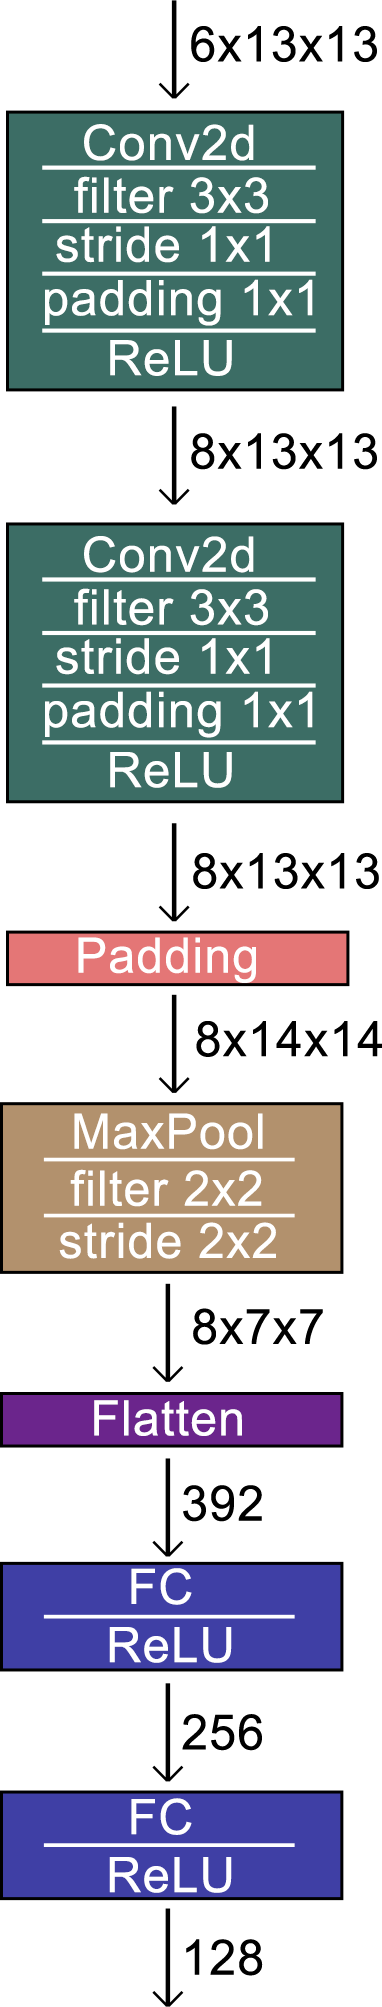
\includegraphics[width=3.0cm, height=15.5cm]{Abbildungen/ConvNet.png}
	\caption[ConvNet]{\\ConvNet}
	\label{fig:ConvNet}
\end{wrapfigure}

Im Rahmen dieser Ausarbeitung soll sich auf eine Netzstruktur konzentriert werden, um die Vergleichbarkeit der einzelnen Algorithmen zu erhöhen. Dennoch müssen, aufgrund des Algorithmus, kleinere Anpassungen an der Netzstruktur vorgenommen werden. Diese werden im weiteren erklärt.\\
Dieses NN stellt dabei einen Kompromiss zwischen Vollständigkeit und Effizienz dar. Wurden in den Papers von \cite{Autonomous_Agents_in_Snake_Game_via_DRL} und \cite{UAV} nur ein einziges großes CNN \ref{sec:Anhang_CNN} genutzt, welche Gefahr läuft viele, für den Spielerfolg, unnötige Informationen zu verarbeiten und eventuelle Probleme mit variablen Spielfeldgrößen zu bekommen, so wird in dieser Ausarbeitung auf ein zweiteilige Netzstruktur gesetzt. Diese besteht aus dem ConvNet und dem Actor-, Critic- oder Q-Head.
Zuerst wird die AV durch zwei Convolutional Layer mit einer ReLU Aktivierungsfunktion geleitet. Dabei erhöht sich die Channel-Anzahl auf acht, wobei eine weitere Erhöhung der Channel-Anzahl aufgrund der bereits sehr stark optimierten AV nicht nötig ist. Die Feature Map wird während dieses Prozesses nicht minimiert, aufgrund des Paddings der Conv2d Layers. Dies soll den Informationsverlust an den Rändern minimieren.  
Danach werden allen Feature Maps eine Null-Zeile und Spalte hinzugefügt (Padding), damit beim Max-Pooling unter der Filtergröße und dem Stride von 2x2, auch die letzten Zeile und Spalte verarbeitet wird. Der Tensor besitzt nun die Form (8x14x14). Nach dem max-pooling besitzt der Tensor, Feature Maps der Größe 7x7. Nach einer Einebnung (Flatten) zu einem eindimensionalen Tensor wird, wird dieser durch zwei weitere Fully Connected Layer (FC) mit einer ReLU Aktivierungsfunktion propagiert. Der resultierende Tensor besitzt die Größe 1x128 und ist ein zwischen Ergebnis, da dieser nun mit der SO verbunden wird (Join).
%eine zeile platz sonst failed die Formartierung
\begin{wrapfigure}{l}{5.1cm}
	\centering
	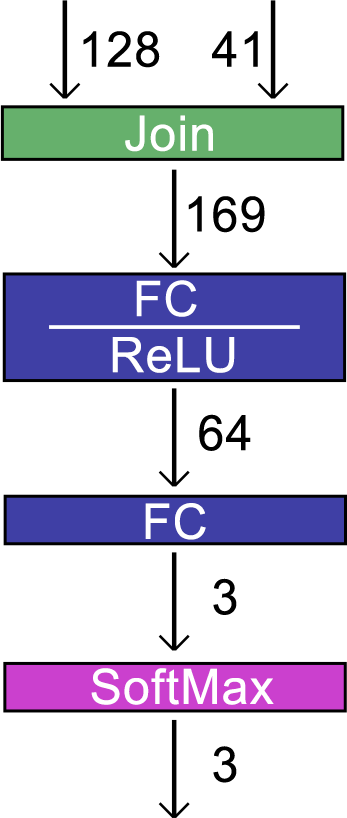
\includegraphics[width=3.0cm, height=8.0cm]{Abbildungen/Actor.png}
	\caption[Actor-Head]{\\Actor-Head}
	\label{fig:Actor_Head}
\end{wrapfigure}

Da das NN in beide Algorithmus-Arten verwendet wird, müssen Netzwerkköpfe für den Actor, Critic und für das Q-Net definiert werden. Alle unterscheiden sich jedoch nur in ihrer Ausgabe. 
Nachdem der Joined Tensor (1x169) durch zwei weitere FC Layer mit ReLU Aktivierungsfunktion propagiert wurde, benötigt der Actor des PPO-Agenten eine Wahrscheinlichkeitsverteilung über alle Actions. Daher auch die Ausgabe von einem Tensor der Größe drei. Um diese Wahrscheinlichkeitsverteilung zu erhalten, wird die SoftMax Funktion angewendet, siehe \ref{fig:Actor_Head}.\\
Der Critic des PPO verwendet hingegen den Critic-Head, siehe \ref{fig:Critic_Q_Head} links. Dieser leitet den Joined Tensor durch ein weiteres FC Layer mit ReLU Aktivierung. Der Resultierende Output wird danach durch ein weiteres FC Layer ohne Aktivierung geleitet. Da der Critic für jeden State die Discounted Sum of Rewards zu bestimmt \ref{sec:Baseline_Estimate}, gibt dieser einen Tensor mit einem einzigen Wert zurück.
Der Q-Net-Kopf ist in seinem Aufbau sehr ähnlich zu dem Critic-Kopf. Da dieser jedoch die Q-Values für jede Aktion im Zustand angeben soll, muss ein Tensor der Größe drei zurückgegeben werden. Von der Struktur des Netzes sind jedoch der Critic- und Q-Net-Kopf gleich, siehe \ref{fig:Critic_Q_Head}.
\begin{figure}[H]
	\centering
	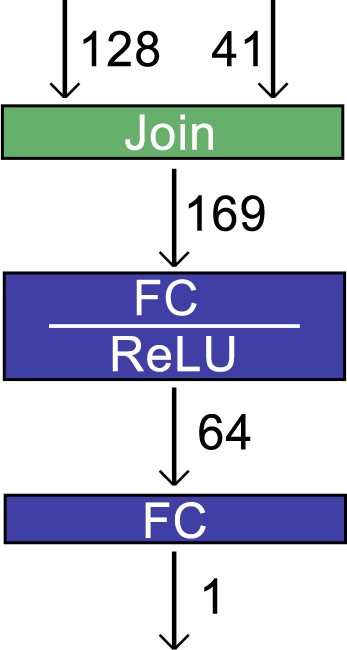
\includegraphics[width=3cm, height=5.2cm]{Abbildungen/Critic.png}
	\hspace{.3\linewidth}% Abstand zwischen Bilder
	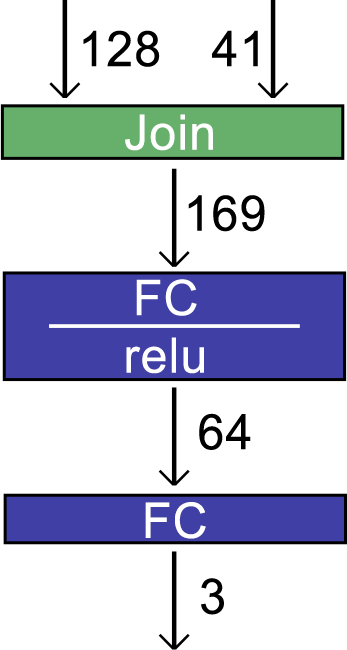
\includegraphics[width=3cm, height=5.2cm]{Abbildungen/QNet.png}
	\caption[Critic- und Q-Net-Head]{Darstellung des Critic-Kopfes (links) und des Q-Net-Kopfes (rechts).}
	\label{fig:Critic_Q_Head}
\end{figure}


\subsection{DQN}
Der DQN Algorithmus und damit auch die Agenten, welche auf dem Algorithmus basieren, bestehen aus drei Komponenten. Diese ermöglichen die Implementierung der Hauptmethoden act und learn.
\begin{figure}[H]
	\centering
	\def\svgscale{0.18}
	\input{Abbildungen/DQN-Agent.pdf_tex}
	\caption[DQN-Agent]{Darstellung des DQN-Agent mit seinen Komponenten.}
	\label{fig:DQN-Agent}
\end{figure}
Diese Hauptmethoden sind in der DQN-Komponente eingebettet, welche die zentrale Instanz des DQN darstellt. In ihr werden zudem die Memory und Q-Network Komponente verwaltet. Des Weiteren werden wichtige Konstanten für den DQN Algorithmus, wie z.B. Gamma (gamma), Epsilon (eps), Epsilon-Dekrementierung (eps\_dec), der minimal Wert für Epsilon (eps\_min), die Batch-Size (batch\_size), die maximale Größe des Memory (max\_mem\_size) und die Lernrate (lr), in der DQN-Komponente gespeichert.\\
Die Memory-Komponente speichert die gesammelten Erfahrungen des DQN-Agenten in einer Ring-Buffer Struktur. Sollte dieser Buffer voll sein, so werden die ältesten Erfahrungen mit den neuen überschrieben.
Die gespeicherten Erfahrungen werden im weiteren Verlauf von der learn Methode abgerufen, um mit ihnen den Lernprozess durchzuführen. Abzuspeichernde Werte, für jeden Schritt, sind dabei die around\_view (AV), die scalar\_obs (SO) die Aktion (action), der Reward (reward), die Information, ob man sich in einem terminalen Zustand befindet (terminal) und die around\_view (AV\_) und scalar\_obs (SO\_) des Nachfolgezustandes. \\
Die Q-Network-Komponente verwaltet das NN (Q-Network). Dieses wird von der act Methode dazu genutzt, um die Aktionen für das Env zu bestimmen. Des Weiteren wird das Q-Network durch die learn Methode aktualisiert, sodass eine höhere Performance erreicht werden kann.

\subsubsection{Aktionsauswahlprozess} \label{sec:Konzept_Aktionsauswahlprozess_DQN}
Zur Bestimmung der nächsten Action wird der act Methode die momentane Obs übergeben.
Diese generiert einen Zufallswert zwischen null und eins, was den Wahrscheinlichkeiten von 0\% bis 100\% entspricht.
Ist der Zufallswert größer als den momentane Epsilon-Wert, so wird die Aktion durch das Q-Network bestimmt. Anderenfalls wird eine zufällige Aktion ausgewählt. Die Bestimmung der Aktion durch das Q-Network geschieht dabei wie folgt.\\
Die around\_view (AV) und die scalar\_obs (SO) werden durch das Q-Network, entsprechende der Ausführungen in \ref{sec:Konzept_Netzstruktur}, geleitet. Dieses gibt einen Tensor der Größe drei wieder, welche die Q-Values der Aktionen turn left (0), turn right (1) und do nothing (2) beinhaltet.
Es wird daraufhin die Aktion gewählt welche dem Index des größten Q-Values entspricht.\\
Sei (0.32, -0.11, 0.45) ein Tensor, welcher vom Q-Network zurückgegeben wurde, dann würde no nothing (2) gewählt werden, da 0.45 der größte Q-Value ist und an Stelle 2 steht.\\
Zum Schluss wir die Aktion zurückgegeben und die Methode terminiert.
\begin{figure}[H]
	\centering
	\def\svgscale{0.13}
	\input{Abbildungen/DQN-Aktionsbestimmung.pdf_tex}
	\caption[DQN-Aktionsbestimmung]{Darstellung der Aktionsbestimmung des DQN-Agent.}
	\label{fig:DQN-Aktionsbestimmung}
\end{figure}

\subsubsection{Lernprozess} \label{sec:Konzept_Lernprozess_DQN}
Der Lernprozess wird über die learn Methode ausgeführt und stellt sich dabei wie folge dar:\\
Zuerst wird überprüft, ob im Memory genügend Experiences (Exp) gespeichert sind, um einen Mini-Batch mit der zuvor definierten batch\_size, zu extrahieren. Sollte dies nicht der Fall sein, wird die Methode terminiert. Anderenfalls wird ein Mini-Batch aus zufälligen Exp ohne Duplikate gebildet.\\
Danach wird der Q-Value bestimmt, welcher zu der abgespeicherten Aktion gehört. Es wird daher $Q(s_i,a_i;\theta_i)$ bestimmt \ref{eq:DQN_Loss}, wobei $s_i$ die Observation (AV und SO), $a_i$ die gewählte Aktion im State $s_i$ und $\theta$ die Netzwerkparameter des Q-Network, darstellten. Dieser wird als Q-Eval definiert.
Als nächstes werden die Q-Values des Nachfolgezustandes (AV\_ und SO\_) bestimmt. Sollte der Nachfolgezustand ein terminaler Zustand sein, so wird der Q-Value auf null gesetzt, da die Q-Values die zu erwartende Discounted Sum of Rewards angeben. In einem terminalen Zustand ist diese gleich null, da keine Zustande mehr Besucht werden können \ref{sec:Q-Learning}.\\
Daraufhin wird der maximale Q-Value bestimmt, mit gamma multipliziert und mit dem erhaltenen Reward addiert. Es wird daher $r(s,a) + \gamma \max_{a'}Q(s',a';\theta_{i-1})$ bestimmt \ref{eq:DQN_Loss}. Dieser Wert wird als Q-Target definiert und entspricht Q-Eval.
Am Ende wird der Mean Squared Error zwischen den Q-Targets und Q-Evals aus dem Mini-Batch gebildet. Auf Basis dieses Fehlers soll das Q-Network mittels Backpropagation und Gradientenverfahren \ref{Backprop_GD} angepasst werden.

\subsection{PPO}
\begin{figure}[H]
	\centering
	\def\svgscale{0.18}
	\input{Abbildungen/PPO-Agent.pdf_tex}
	\caption[PPO-Agent]{Darstellung des PPO-Agent mit seinen Komponenten.}
	\label{fig:PPO-Agent}
\end{figure}
Der PPO Algorithmus und damit auch die Agenten, welche auf diesem Algorithmus basieren, bestehen aus vier Komponenten. Diese ermöglichen die Implementierung der Hauptmethoden act und learn.\\
Diese Hauptmethoden sind in der PPO-Komponente eingebettet, welche die zentrale Instanz des DQN darstellt. In ihr werden zudem die Memory-, Actor- und die Critic-Komponenten verwaltet. Des Weiteren werden wichtige Konstanten für den PPO Algorithmus, wie z.B. Gamma (gamma), der Epsilon-Clip-Wert (eps\_clip) \ref{sec:Surrogate_Objectives}, Anzahl der Trainingsläufe pro Datensatz (K\_Epochs), die Lernrate (lr) und weitere Statische Konstanten, in der PPO-Komponente gespeichert.\\
Die Memory-Komponente speichert die gesammelten Erfahrungen des PPO-Agenten. Diese werden im weiteren Verlauf von der learn Methode abgerufen, um mit ihnen den Lernprozess durchzuführen. Abzuspeichernde Werte, für jeden Schritt, sind dabei die around\_view (AV), die scalar\_obs (SO) die Aktion (action), der Reward (reward), die Information, ob man sich in einem terminalen Zustand befindet (terminal) und die logarithmierte Wahrscheinlichkeit der Aktion (log\_prob). \\
Die Actor-Komponente verwaltet das Actor-NN. Dieses wird von der act Methode dazu genutzt, um die Aktionen für das Env zu bestimmen. Des Weiteren wird das Actor-NN durch die learn Methode aktualisiert, sodass eine höhere Performance erreicht werden kann.\\
Die Critic-Komponente verwaltet das Critic-NN. Dieses wird einzig von der learn Methode verwendet, um die erwartete Discounted Sum of Rewards zu bestimmen. mit dieser wird im Trainingsverlauf der Value-Loss bestimmt \ref{eq:Value_Loss}.

\subsubsection{Aktionsauswahlprozess} \label{sec:Konzept_Aktionsauswahlprozess_PPO}
Der Aktionsauswahlprozess wird durch die act Methode in der PPO-Komponente angestoßen, welche die around\_view und die scalar\_obs übergeben bekommt. Dieser werden sogleich durch das Actor-NN, welches sich in der Actor-Komponente befindet, propagiert. Der vom Actor-NN ausgegebene Tensor der Größe drei, beinhaltet eine Wahrscheinlichkeitsverteilung. Auf Basis dieser Verteilung wird die nächste Aktion bestimmt.\\
Sei (0.05, 0.05, 0.9) die Wahrscheinlichkeitsverteilung über alle Aktionen. bestimmte man 100 Aktionen unter dieser Verteilung, so würde durchschnittlich 90-mal die Aktion zwei gewählt werden. Aktion null und eins nur rund fünfmal.\\
Zum Schluss wird die Aktion zurückgegeben und die act Methode wird terminiert.

\subsubsection{Lernprozess} \label{sec:Konzept_Lernprozess_PPO}
Der Lernprozess des PPO wird durch die learn Methode angestoßen. Dabei wird wie folgt verfahren.\\
Zu Beginn werden die Erfahrungen, aus den gespielten Spielen, aus dem Memory (Replay-Buffer) extrahiert. Der Memory bzw. Replay Buffer befindet sich in der Memory-Komponente.\\
Um den Return \ref{sec:Return} zu erhalten, werden die einzelnen Rewards aus dem Memory, welche extrahiert worden sind, diskontiert. Sollte der Reward dabei aus einem terminalen Zustand entstanden sein, so wird dieser auf null gesetzt, da der Return der diskontierten Summe aller Rewards bis zum Ende der Spielepisode entspricht. Nach einem terminalen Zustand werden keine weiteren zustände besucht, sodass keine neuen Rewards gesammelt werden können und daher der Return gleich null ist.\\
Um ein gleichmäßigeres Lernen zu unterstützen, werden die Rewards in Anschluss noch normalisiert.
Danach wird die folgende Prozedur (K\_epochs) mal ausgeführt, um das NN zu trainieren. Danach terminiert die learn Methode.\\
Als nächstes werden die logarithmierte Wahrscheinlichkeiten für die gespeicherten Aktionen $a_i$ $\pi_{\theta}(a_{t}|s_{t})$ bestimmt \ref{sec:Probability_Ratio}. Dazu werden die aus dem Memory entnommenen AVs (around\_view) und SOs (scalar\_obs) durch das Actor- und Critic-NN propagiert. Anschließend werden die logarithmierte Wahrscheinlichkeiten für die Aktionen bestimmt und zusammen mit den Baseline Estimates \ref{sec:Baseline_Estimate} und den Entropien der Wahrscheinlichkeitsverteilungen \ref{sec:PPO_Training_Objective_Function} zurückgegeben.\\
Daraufhin werden die Probability Ratios aus der eben bestimmten logarithmierte Wahrscheinlichkeiten und den alten logarithmierte Wahrscheinlichkeiten des Memories bestimmt \ref{sec:Probability_Ratio}.
Nachfolgend werden die Advantages durch Subtraktion der Returns mit den Baseline Estimates berechnet $\hat{A}_{t}(s, a) = R_{t} - b(s_{t})$ \ref{sec:Advantages}.\\
Des Weiteren werden als nächstes die Surrogate Objective Losses Surr1: $r_{t}(\theta) \hat{A}_{t}(s, a)$ und Surr2: $\text{clip}(r_{t}(\theta), 1 - \epsilon, 1 + \epsilon) \hat{A}_{t}(s, a)$ bestimmt \ref{sec:Surrogate_Objectives}, mit welchen der Actor-Loss $L^\text{CLIP}_{t} (\theta) = \mathbb{\hat{E}}_{t} [ \min(r_{t}(\theta) \hat{A}_{t}(s, a), \text{clip}(r_{t}(\theta), 1 - \epsilon, 1 + \epsilon) \hat{A}_{t}(s, a))]$ berechnen wird.
Um zum Schluss den gesamt Loss des PPO zu bestimmen zu können, wird zusätzlich noch der Value-Loss $L^{\text{VF}}_{t} = (V_{\theta}(s_{t})-V_{t}^{targ})^2 \text{ wobei } V_{t}^{targ} = r_{t}(\theta)$ und Entropy-Loss bestimmt \ref{sec:PPO_Training_Objective_Function}. Diese wenden dann alle zusammengerechnet, entsprechend der Formel: 
$L^\text{PPO}_{t} (\theta) = L^\text{CLIP + VF + S}_{t} (\theta) = \mathbb{\hat{E}}_{t} [L^{\text{CLIP}}_{t}(\theta) - c_{1}L^{\text{VF}}_{t} + c_{2}S[\pi_{\theta}](s_{t})]$ \ref{sec:PPO_Training_Objective_Function}.\\
Das Actor- und Critic-NN werden mit dem Loss unter Zuhilfenahme von Backpropagation und Gradientenverfahren aktualisiert.

\subsection{Vorstellung der zu untersuchenden Agenten}
Ein zentraler Aspekt eines Vergleiches von verschiedenen RL-Agenten ist die genaue Definition dieser einzelnen. 
Basierende auf den Grundlagen \ref{sec:Agent} soll in diesem Abschnitt die zu vergleichenden Agenten vorgestellt werden.\\
Da die ausgewählten Hyperparameter einen immensen Einfluss auf das Verhalten der Agenten besitzen, ist ein Vergleich zwischen DQN und PPO Agenten mit wahllos gewählten Hyperparametern folglich wenig aussagekräftig. Darum sollen im weiteren die Wahl der Hyperparameter der Agenten hier begründet werden.\\
\\Wie bereits in der Abbildung \ref{fig:Vorgehen} zu erkennen ist, sollen 6 Agenten definiert und miteinander verglichen werden.
\begin{figure}[H]
	\centering
	\def\svgscale{0.102}
	\chapter{Agenten}
Ein zentraler Aspekt der eines Vergleiches von verschiedenen RL-Agenten ist die genaue Definition der einzelnen Agenten. Basierende auf den Grundlagen \ref{sec:Agent} soll in diesem Kapitel der Begriff vervollständigt und die zu vergleichenden Agenten sollen vorgestellt werden.\\
Erste statistische Erhebungen haben gezeigt, dass die ausgewählten Hyperparameter einen immensen Einfluss auf das Verhalten der Agenten haben. Bestätigt wird diese Aussage durch die Quelle \cite{Sutton1998}. Ein Vergleich zwischen DQN und PPO mit wahllos gewählten Hyperparametern ist folglich wenig aussagekräftig. Daher ist auch die Definition des Begriffs Agent, welcher nur zwischen DQN und PPO diffenenziert, unzureichend.\\
\\Angebracht wäre eine neuer erweiterte Definition des Begriffs Agent für diese Ausarbeitung. Diese soll um den entscheidenen Faktor der Hyperparameter erweitert werden. Ein Agent wird daher nicht mehr alleinig durch seine Art (Q-Learning oder Policy Gradient bzw. DQN oder PPO) definiert, sondern ebenfalls durch die ausgewählten Hyperparameter.Eine Analogie aus dem Tierreich sollte hier Klarheit verschaffen.\\
\\Im Tierreich gibt es Hunde und Katzen. Diese stellen die RL-Klassen, wie z.B. Q-Learning- oder Policy Gradient Verfahren, dar. Sieht man jedoch genauer hin, so unterscheiden sich die Hunde und Katzen durch ihre jeweiligen Rassen, wie z.B. Pudel und Dalmatiner bei den Hunden und Maine Coons und Norwegische Waldkatzen bei den Katzen. Diese stellen die Algorithmusklassen, wie z.B. DQN oder PPO, dar. Dennoch unterscheiden sich auch Hunde und Katzen der selben Rasse untereinander, nämlich in ihrer DNS. Diese stellt die letzte Differenzierungsebene der Agenten dar. Im Sachzusammenhang stellen die Hyperparameter und Attribute, wie beispielsweise die Netzstruktur, die DNS eines Agenten dar.\\
Soll nun also ein Vergleich zwischen verschiedenen Agenten vollzogen werden, so gilt es als erstes die einzelnen Agenten zu definieren, daher ihre RL-Klasse, Algorithmusklasse und Hyperparameter zu bestimmen.
 
	\caption[Agenten]{Darstellung der zu untersuchenden Agenten.}
	\label{fig:Agenten}
\end{figure}
Der erste Agent PPO-01 soll ein langsamer aber stetiger Lerner sein. Mit einer ACTOR-LR von 2e-4 und einer CRITC-LR von 4e-4 wurden Lernraten gewählt, welche, spezifisch für diese Netzstruktur, im Mittelfeld liegen. Ein hoher Wert für GAMMA von 0.99 sorgt für ein zukunftsorientiertes Lernen. Mit einem K\_EPOCHS-Wert von acht wird das Lernen weiter verlangsamt und verstetigt. Damit der PPO-01 keine zu großen Aktualisierungen der Netze unternimmt, wurde EPS\_CLIP auf 0.15 gesetzt, was, verglichen mit der Literatur \cite[S. 6]{PPO}, recht niedrig ist.\\
\\ Der PPO-02 soll ein schnell lernendes Verhalten zeigen. Zu diesem Zweck wurden zwar niedrige Lernraten von des Actors von 1e-4 und des Critics von 2.5e-4 gewählt, jedoch sorgt relativ großer K\_EPOCHS-Wert von zwölf für ein stärkeres Aktualisieren der Netzwerkparameter von Actor und Critic. Dies wird ebenfalls durch den EPS\_CLIP-Wert von 0.25 unterstützt, welcher, nach der PPO Literatur \cite[S. 6]{PPO}, höher als der Durchschnittswert ist. Der GAMMA-Wert von 0.95 bestärkt zudem den schnelleren Lernerfolg, aufgrund der Kurzzeitpräferenz des Agenten.\\
\\PPO-03 soll ein Kompromiss zwischen schnellen Lernen und stetigem Fortschritt sein. Mit mittleren Lernraten von des Actors und Critics von 1.5e-4 bzw. 2.5e-4 sollte ein schneller und zugleich stetiger Lernfortschritt erzielt werden. Der GAMMA-Wert von 0.97 soll als Kompromiss zwischen Kurz- und Weitsichtigkeit dienen. Auch die Werte von K\_EPOCHS mit zehn und EPS\_CLIP von 0.2 werden in der Literatur \cite[Anhang A]{PPO} empfohlen und stellt ein gutes Mittelmaß dar.\\
\\Der DQN-01 ist wieder als langsamer Lerner gedacht. Mit einer mittleren LR on (LR = 0.9e-4) und einem großen GAMMA-Wert von 0.99, wird ein stetiges und zukunftsorientiert Lernen bestärkt. Eine BATCH\_SIZE und Memory-Size (MAX\_MEM\_SIZE) 64 und 2**15, soll zudem das Lernen verlangsamen. Geringe Werte für Eps\_Dec und EPS\_MIN von 5e-6 und 0.01 sollen die Neugierde des Agenten zu Beginn stärken und die Wahl von Zufallsaktionen in späteren Trainingsphasen senken.\\
\\DQN-02 ist wieder als Schnelllerner konzipiert worden. Eine vergleichsweise hohe Lernrate (LR) von 1.5e-4 in Verbindung mit einem mittleren bis kleinen Wert für Gamma von 0.95 soll einen schnellen Lernfortschritt generieren. Dies wird durch die niedrige Memory-Size (MAX\_MEM\_SIZE) von 2**11 und die große Epsilon-Dekrementierung (EPS\_DEC) von 1e-5 verstärkt. Auch sorgt der verhältnismäßig große Wert für EPS\_MIN von 0.05 für eine schnellerer Exploration und damit für ein schnelles Lernen.\\
\\ Der DQN-03 besitzt die folgenden Hyperparameter, LR = 1e-4, GAMMA = 0.97, BATCH\_SIZE = 64, MAX\_MEM\_SIZE = 2**12, 
EPS\_DEC = 8e-6 und EPS\_END = 0.025 und ist mit dieser Kombination an Parametern ein mittelfristiger Lerner.

\section{Optimierungen}
In diesem Abschnitt werden die anzuwendenden Optimierungen vorgestellt und erklärt, welche nach dem Baseline-Vergleich die Leistung in den einzelnen Evaluationskategorien noch weiter verstärken soll. Zu diesem Zweck sollen vier Optimierungen auf die Baseline Agenten (Agenten ohne Optimierungen) angewendet werden, welche aus einer verwandten Arbeit \ref{sec:Paper_1} und eigenen Ideen stammten.\\
\\ Die Optimierungen welche aus dem Paper "`UAV Autonomous Target Search Based on Deep Reinforcement Learning in Complex Disaster Scene"' \cite{UAV} konnten bezüglich ihrer Qualität nicht überzeugen. Das aper hat als Optimierung eine neue Reward Funktion vorgestellt die sehr einfach gehalten ist und wenige Spielfaktoren mit in die Berechnung des Rewards mit einfließen lasst  sodass zwei Optimierungen aus dem Paper "`Autonomous Agents in Snake Game via Deep Reinforcement Learning"' \cite{Autonomous_Agents_in_Snake_Game_via_DRL} für den folgenden Vergleich ausgewählt wurden.

\subsection{Optimierung A - Dual Experience Replay} \label{sec:Konzept_Optimierung01}
Die Idee für Dual Experience Replay oder auch hier Splited Memory genannt, stammt aus der Arbeit "`Autonomous Agents in Snake Game via Deep Reinforcement Learning"' \cite{Autonomous_Agents_in_Snake_Game_via_DRL} und wurde in \ref{sec:Paper_1} bereits erwähnt.\\
Diese Optimierung zielt darauf ab, den Replay Buffer (Memory) zu zweiteilen, sodass ein Mem1 und Mem2 entstehen. In Mem1 werden ausschließlich Erfahrungen gespeichert, welche einen Reward vorweisen können, der größer als ein vordefinierter Grenzwert ist. In Mem2 werden alle übrigen Erfahrungen gespeichert. Diese Aufteilung zielt darauf ab, dass zu beginn ein größerer Anteil an guten Erfahrungen für das Lernen verwendet wird, um das Lerntempo und die Stabilität zu erhöhen. Den Verfassern schwebt ein Verhältnis von (80\% guten und 20 \% schlechteren Erfahrungen vor). Dieses Verhältnis normalisiert sich über die Trainingszeit, daher zum Verhältnis von (50\% zu 50\%).\\
Problematisch ist jedoch die erfahrungsorientierte Aufteilung, da diese für den PPO nur schlecht umsetzbar ist.\\
Alternativ kann die Sortierung nicht auf Erfahrungsbasis, sondern Episoden basiert geschehen. Es werden daher die besten Spielepisoden, gemessen an ihren Scores, in die Memories einsortiert.\\
Zu diesem Zweck wird eine weitere Memory-Art in den Memory-Komponenten des DQN und PPO definiert, welchen diese beschriebene Funktionalität bereitstellt. Diese trägt den Namen Splited-Memory\\
Beim DQN Memory wird zusätzlich darauf geachtet, dass beim Einfügen einer ganzen Episode an Erfahrungen die Ring-Buffer Eigenschaften des Memory erhalten bleiben. Beim Memory des PPO ist dies nicht nötig.


\subsection{Optimierung B - Joined Reward Function} \label{sec:Konzept_Optimierung02}
Die Joined Reward Function wurde im Paper "`Autonomous Agents in Snake Game via Deep Reinforcement Learning"' \cite{Autonomous_Agents_in_Snake_Game_via_DRL} vorgestellt und in \ref{sec:Paper_1} erklärt. Sie setzt sich aus drei Teilen zusammen. Die Basis bildet ein Distanz Reward, welcher abhängig von der Distanz und Schwanzlänge ist. Um unerwünschte Lerneffekte, von beispielsweise der Neuerzeugung eines Apfels, zu verhindern werden diese Erfahrungen aus dem Memory gelöscht, was die Training Gap Strategy und den zweiten Teil der Reward Funktion darstellt. Zur Verstärkung des Pathfindings wird die Timeout Strategy angewendet, welche den Agenten für nicht zielgerichtetes Verhalten, wie z.B. das unnötige Umherlaufen, bestraft.\\
Die Implementierung dieser neuen Reward Funktion findet in der Reward-Komponente statt. Dabei wird der Reward wie folgt berechnet:
\begin{align}
	r_{distanz}(dis, len, size) = \frac{10}{dis} \times \frac{len}{size}
\end{align}
$dis$ stellt die Distanz gemessen mit der Euklidischen Norm dar, $len$ ist die Länge der Snake und $size$ ist die Größe des Spielfeldes (bei einer Spielfeldform von 8x8 ergibt sich eine Größe von 64).\\ Da die Training Gap Strategy zu Problemen beim PPO führen würde, wird diese nicht beachtet. Die Timeout Strategy wird in abgewandelter Form implementiert. Dies geschieht nach folgender Formel:
\begin{align}
	r_{timeout}(steps, len) = \frac{1}{100} \times \frac{steps}{len}
\end{align}
$steps$ beschreibt die Anzahl an Schritten, welche seit dem letzten Konsum eines Apfels gelaufen worden sind. 
Die Joined Reward Function lautet daher: $r_{res}(dis, len, size, steps) = 	r_{distanz}(dis, len, size) - r_{timeout}(steps, len)$.

\subsection{Optimierung C - Anpassung der Lernrate} \label{sec:Konzept_Optimierung03}
Die dritte Optimierung versucht das Lernen des Agenten durch das stetige Anpassen der Lernrate (LR) zu verbessern. 
Die Lernrate wird immer dann mit 0.95 multipliziert und als neue LR gesetzt, sobald keine Performance Steigerung in den letzten 200 Schritten erfolgt ist.

\subsection{Optimierung D - Parameteraddition zu den Netzwerken} \label{sec:Konzept_Optimierung04}
Die vierte Optimierung versucht durch das Hinzufügen von Parametern zu den Netzwerken des Actors, Critics und des Q-Networks die Performance zu steigern. Konkret sollen die Parameter der Netzwerke ansatzweise verdoppelt werden. Natürlich bietet sich dies nicht an jeder Stelle der Netzstruktur an, daher werden nur bestimmte Layer des NN von der Optimierung betroffen sein. An der Struktur des NN wird jedoch nichts verändert. Die optimierte Netzstruktur ist im Anhang \ref{fig:ConvNetOptimized} dargestellt. 


\section{Datenerhebung und Verarbeitung} \label{sec:Konzept_Datenerhebung_Verarbeitung}
In diesem Abschnitt soll die Datenerhebung näher thematisiert werden. Zu diesem Zweck wird soll zuerst die Hauptmethode näher erklärt werden, welche Agenten und Env mit einander interagieren lässt. Danach wird die Statistik-Komponente mit ihren Methoden vorgestellt.

\subsection{Datenerhebung} \label{sec:Konzept_Datenerhebung}
Die Hauptmethode oder auch main Methode genannt, implementiert den eigentlichen Spiel und Trainingsablauf. Die main Methde der Agenten ist außerhalb der der Komponenten der Agenten zu finden, da beide Algorithmus-Arten und ihren Agenten, die gleiche Standardisierte Schnittstelle verwenden. \ref{sec:Anforderungen_Schnittstelle}. 
Um den Spiel- und Trainingsablauf durchzuführen, wird die train Methode der DQN bzw PPO Agenten aufgerufen, welche wichtige Hyperparameter des Ablaufs, wie z.B. die zu absolvierenden Trainingsspiele (N\_ITERATIONS), die Spielfeldgröße (BOARD\_SIZE) und weitere Agenten spezifische Hyperparameter, übergeben bekommt.\\
Um einen angemessenen Zeitraum für das Lernen zu schaffen soll 30.000 Spiele (N\_ITERATIONS) für einen Trainingslauf gespielt werden. DieSpielfeldgröße soll dabei standardmäßig bei (8x8) liegen.\\
Bei der Datenerhebung ist streng zwischen Spiel- und Trainingsdaten zu unterscheiden, wobei die Spieldaten aus einfachen Spielabläufen und die Trainingsdaten aus den Trainingsabläufen stammen. Die Trainingsdaten werden wie folgt erhoben.\\
Zu Beginn werden die Datenhaltungsobjekt apples, wins, time, (eps für DQN), steps initialisiert, welche für jedes absolvierte Training die, dem Namen des Objektes entsprechenden, Werte speichert. Nach der weiteren Erstellung des Agenten und Environments startet der Spielverlauf.\\
Dabei wird wie in \ref{sec:Funktionsweise} vorgegangen. Der Agent erhält eine Obs, bestimmt seine Action und diese wird sogleich im Env ausgeführt. Danach werden die neue Obs sowie Reward und weitere Statusinformationen, wie z.B. der Lebensstatus (done bzw. terminal) usw., ausgegeben. Diese Daten werden im Memory des jeweiligen Agenten für das sich anschließende Training gespeichert. Dieses wird wie in DQN-Lernprozess \ref{sec:Konzept_Lernprozess_DQN} bzw. PPO-Lernprozess \ref{sec:Konzept_Lernprozess_PPO} durchgeführt. Danach werden die oben genannten Datenhaltungslisten aktualisiert und die Prozedur beginnt von neuem. Wenn diese N\_ITERATIONS Spiele alle absolviert wurden werden die Erhobenen Daten weiter in der Statistik-Komponente verarbeitet \ref{sec:Konzept_Datenverarbeitung}.\\
Die Datenerhebung für Spieldaten findet annähernd auf die gleiche Weise statt. Jedoch werden die Daten in nicht nach jedem Trainingslauf entnommen, sondern nach jeder Spielepisode. Bei den Daten handelt es sich um die gleichen wie in der oben erwähnten Datenerhebung für Trainingsdaten. Diese werden dann ebenfalls der Statistik-Komponente übergeben \ref{sec:Konzept_Datenverarbeitung}.

\subsection{Datenverarbeitung und Erzeugung von Statistiken} \label{sec:Konzept_Datenverarbeitung}
Nach der Erstellung der Trainings- und Spieldaten für jeden Agenten, wenden diese Daten entsprechend der Evaluationskriterien verarbeitet \ref{tab:Kriterien}. Diese Verarbeitung sieht wie folgt aus.\\
Die Performance wird anhand der gefressenen Äpfel gemessen. Das Datenobjekt apples besitzt diese Daten für jeden Trainingsdurchlauf.\\
Die Effizienz errechnet sich aus der Anzahl der gefressenen Äpfel (apples) dividiert durch die gegangenen Schritten (steps). Es entsteht daher die Apfel pro Schritt Rate.\\
Die Robustheit wird mit Hilfe von Spieldaten bestimmt. Dabei wird ein trainierter Agent auf einem Spielfeld mit variabler Größe spielen. Die Robustheit wird danach gleich der Performance gemessen. Es werden daher die gefressenen Äpfel (apples) in der neuen Umgebung gemessen. Die Spielfeldgröße soll dabei zwischen (6x6) bis zu (12x12) liegen. Für die Erhebung werden wie beim Trainingsprozess 30.000 Spiele gespielt.\\
Die Siegrate wird mit Hilfe der Wins bestimmt. Dabei werden die Siege der jeweils zehn letzten Spiele zusammenaddiert und durch die Trainingsspiel dividiert, sodass die Rate Siege der letzten zehn Spiele pro Spiel entsteht.\\
Die Spielzeit berechnet sich aus der vergangenen Zeit für ein Trainingsspiel pro Trainingsspiel.\\
\\Da bei 30.000 gespielten Spielen für jedes Evaluationskriterien gleich viele Werte entstehen, jedoch die Statistik nur eine gewisse Bildgröße besitzen kann, sollen jeweils 10 dieser errechneten Werte zu einem, mit Hilfe der Durchschnitts-, Max- und Min-Funktion, zusammen gefasst werden. Dies soll die Lesbarkeit der Grafiken verbessern und Schwankungen minimieren. Die Statistiken besitzen daher 3.000 (30.000 / 10 = 3.000) Datenpunkte.\\
Diese Datenpunkte werden für alle Agenten eines Vergleiches pro Funktion (Durchschnitts-, Max- und Min-Funktion) aufgetragen. Es entstehen daher pro Datensatz aller Agenten drei Grafiken welche die Minima, Maxima und den Durchschnitt der letzten 10 Datenpunkte der Evaluationskriterien wiedergibt.\\
Eine nähere Darstellung wird im Kapitel Implementierung geliefert \ref{chap:Implementierung}.
